% Options for packages loaded elsewhere
\PassOptionsToPackage{unicode}{hyperref}
\PassOptionsToPackage{hyphens}{url}
%
\documentclass[
]{article}
\title{Causal Impact Analysis on Listing Level Pricing Test}
\author{}
\date{\vspace{-2.5em}}

\usepackage{amsmath,amssymb}
\usepackage{lmodern}
\usepackage{iftex}
\ifPDFTeX
  \usepackage[T1]{fontenc}
  \usepackage[utf8]{inputenc}
  \usepackage{textcomp} % provide euro and other symbols
\else % if luatex or xetex
  \usepackage{unicode-math}
  \defaultfontfeatures{Scale=MatchLowercase}
  \defaultfontfeatures[\rmfamily]{Ligatures=TeX,Scale=1}
\fi
% Use upquote if available, for straight quotes in verbatim environments
\IfFileExists{upquote.sty}{\usepackage{upquote}}{}
\IfFileExists{microtype.sty}{% use microtype if available
  \usepackage[]{microtype}
  \UseMicrotypeSet[protrusion]{basicmath} % disable protrusion for tt fonts
}{}
\makeatletter
\@ifundefined{KOMAClassName}{% if non-KOMA class
  \IfFileExists{parskip.sty}{%
    \usepackage{parskip}
  }{% else
    \setlength{\parindent}{0pt}
    \setlength{\parskip}{6pt plus 2pt minus 1pt}}
}{% if KOMA class
  \KOMAoptions{parskip=half}}
\makeatother
\usepackage{xcolor}
\IfFileExists{xurl.sty}{\usepackage{xurl}}{} % add URL line breaks if available
\IfFileExists{bookmark.sty}{\usepackage{bookmark}}{\usepackage{hyperref}}
\hypersetup{
  pdftitle={Causal Impact Analysis on Listing Level Pricing Test},
  hidelinks,
  pdfcreator={LaTeX via pandoc}}
\urlstyle{same} % disable monospaced font for URLs
\usepackage[margin=1in]{geometry}
\usepackage{color}
\usepackage{fancyvrb}
\newcommand{\VerbBar}{|}
\newcommand{\VERB}{\Verb[commandchars=\\\{\}]}
\DefineVerbatimEnvironment{Highlighting}{Verbatim}{commandchars=\\\{\}}
% Add ',fontsize=\small' for more characters per line
\usepackage{framed}
\definecolor{shadecolor}{RGB}{248,248,248}
\newenvironment{Shaded}{\begin{snugshade}}{\end{snugshade}}
\newcommand{\AlertTok}[1]{\textcolor[rgb]{0.94,0.16,0.16}{#1}}
\newcommand{\AnnotationTok}[1]{\textcolor[rgb]{0.56,0.35,0.01}{\textbf{\textit{#1}}}}
\newcommand{\AttributeTok}[1]{\textcolor[rgb]{0.77,0.63,0.00}{#1}}
\newcommand{\BaseNTok}[1]{\textcolor[rgb]{0.00,0.00,0.81}{#1}}
\newcommand{\BuiltInTok}[1]{#1}
\newcommand{\CharTok}[1]{\textcolor[rgb]{0.31,0.60,0.02}{#1}}
\newcommand{\CommentTok}[1]{\textcolor[rgb]{0.56,0.35,0.01}{\textit{#1}}}
\newcommand{\CommentVarTok}[1]{\textcolor[rgb]{0.56,0.35,0.01}{\textbf{\textit{#1}}}}
\newcommand{\ConstantTok}[1]{\textcolor[rgb]{0.00,0.00,0.00}{#1}}
\newcommand{\ControlFlowTok}[1]{\textcolor[rgb]{0.13,0.29,0.53}{\textbf{#1}}}
\newcommand{\DataTypeTok}[1]{\textcolor[rgb]{0.13,0.29,0.53}{#1}}
\newcommand{\DecValTok}[1]{\textcolor[rgb]{0.00,0.00,0.81}{#1}}
\newcommand{\DocumentationTok}[1]{\textcolor[rgb]{0.56,0.35,0.01}{\textbf{\textit{#1}}}}
\newcommand{\ErrorTok}[1]{\textcolor[rgb]{0.64,0.00,0.00}{\textbf{#1}}}
\newcommand{\ExtensionTok}[1]{#1}
\newcommand{\FloatTok}[1]{\textcolor[rgb]{0.00,0.00,0.81}{#1}}
\newcommand{\FunctionTok}[1]{\textcolor[rgb]{0.00,0.00,0.00}{#1}}
\newcommand{\ImportTok}[1]{#1}
\newcommand{\InformationTok}[1]{\textcolor[rgb]{0.56,0.35,0.01}{\textbf{\textit{#1}}}}
\newcommand{\KeywordTok}[1]{\textcolor[rgb]{0.13,0.29,0.53}{\textbf{#1}}}
\newcommand{\NormalTok}[1]{#1}
\newcommand{\OperatorTok}[1]{\textcolor[rgb]{0.81,0.36,0.00}{\textbf{#1}}}
\newcommand{\OtherTok}[1]{\textcolor[rgb]{0.56,0.35,0.01}{#1}}
\newcommand{\PreprocessorTok}[1]{\textcolor[rgb]{0.56,0.35,0.01}{\textit{#1}}}
\newcommand{\RegionMarkerTok}[1]{#1}
\newcommand{\SpecialCharTok}[1]{\textcolor[rgb]{0.00,0.00,0.00}{#1}}
\newcommand{\SpecialStringTok}[1]{\textcolor[rgb]{0.31,0.60,0.02}{#1}}
\newcommand{\StringTok}[1]{\textcolor[rgb]{0.31,0.60,0.02}{#1}}
\newcommand{\VariableTok}[1]{\textcolor[rgb]{0.00,0.00,0.00}{#1}}
\newcommand{\VerbatimStringTok}[1]{\textcolor[rgb]{0.31,0.60,0.02}{#1}}
\newcommand{\WarningTok}[1]{\textcolor[rgb]{0.56,0.35,0.01}{\textbf{\textit{#1}}}}
\usepackage{graphicx}
\makeatletter
\def\maxwidth{\ifdim\Gin@nat@width>\linewidth\linewidth\else\Gin@nat@width\fi}
\def\maxheight{\ifdim\Gin@nat@height>\textheight\textheight\else\Gin@nat@height\fi}
\makeatother
% Scale images if necessary, so that they will not overflow the page
% margins by default, and it is still possible to overwrite the defaults
% using explicit options in \includegraphics[width, height, ...]{}
\setkeys{Gin}{width=\maxwidth,height=\maxheight,keepaspectratio}
% Set default figure placement to htbp
\makeatletter
\def\fps@figure{htbp}
\makeatother
\setlength{\emergencystretch}{3em} % prevent overfull lines
\providecommand{\tightlist}{%
  \setlength{\itemsep}{0pt}\setlength{\parskip}{0pt}}
\setcounter{secnumdepth}{-\maxdimen} % remove section numbering
\ifLuaTeX
  \usepackage{selnolig}  % disable illegal ligatures
\fi

\begin{document}
\maketitle

\begin{Shaded}
\begin{Highlighting}[]
\FunctionTok{library}\NormalTok{(CausalImpact)}
\end{Highlighting}
\end{Shaded}

\begin{verbatim}
## Loading required package: bsts
\end{verbatim}

\begin{verbatim}
## Loading required package: BoomSpikeSlab
\end{verbatim}

\begin{verbatim}
## Loading required package: Boom
\end{verbatim}

\begin{verbatim}
## Loading required package: MASS
\end{verbatim}

\begin{verbatim}
## 
## Attaching package: 'Boom'
\end{verbatim}

\begin{verbatim}
## The following object is masked from 'package:stats':
## 
##     rWishart
\end{verbatim}

\begin{verbatim}
## 
## Attaching package: 'BoomSpikeSlab'
\end{verbatim}

\begin{verbatim}
## The following object is masked from 'package:stats':
## 
##     knots
\end{verbatim}

\begin{verbatim}
## Loading required package: zoo
\end{verbatim}

\begin{verbatim}
## 
## Attaching package: 'zoo'
\end{verbatim}

\begin{verbatim}
## The following objects are masked from 'package:base':
## 
##     as.Date, as.Date.numeric
\end{verbatim}

\begin{verbatim}
## Loading required package: xts
\end{verbatim}

\begin{verbatim}
## 
## Attaching package: 'bsts'
\end{verbatim}

\begin{verbatim}
## The following object is masked from 'package:BoomSpikeSlab':
## 
##     SuggestBurn
\end{verbatim}

\begin{Shaded}
\begin{Highlighting}[]
\FunctionTok{library}\NormalTok{(zoo)}

\DocumentationTok{\#\#\#\#\#\#\#\#\#\#\#\#\#\#\#\#\#\#\#\#\#\#\#\#\#\#\#\#\#\#\#\#\#\#\#\#\#\#\#\#\#\#\#\#\#\#\#\#\#\#\#\#\#\#\#\#\#\#}
\CommentTok{\# Experiment overall analysis}
\DocumentationTok{\#\#\#\#\#\#\#\#\#\#\#\#\#\#\#\#\#\#\#\#\#\#\#\#\#\#\#\#\#\#\#\#\#\#\#\#\#\#\#\#\#\#\#\#\#\#\#\#\#\#\#\#\#\#\#\#\#\#}

\DocumentationTok{\#\#\#\#\#\#\# T1 \#\#\#\#\#\#}
\CommentTok{\# GMV }
\NormalTok{gmv\_t1 }\OtherTok{\textless{}{-}} \FunctionTok{read.csv}\NormalTok{(}\StringTok{"weekly\_pv\_gmv\_t1.csv"}\NormalTok{, }\AttributeTok{sep =} \StringTok{\textquotesingle{},\textquotesingle{}}\NormalTok{,}\AttributeTok{header =} \ConstantTok{TRUE}\NormalTok{)}
\NormalTok{gmv\_t1 }\OtherTok{\textless{}{-}}\NormalTok{ gmv\_t1[}\FunctionTok{order}\NormalTok{(gmv\_t1}\SpecialCharTok{$}\NormalTok{period, }\AttributeTok{decreasing=}\ConstantTok{TRUE}\NormalTok{), ]}
\NormalTok{gmv\_t1 }\OtherTok{\textless{}{-}}\NormalTok{ gmv\_t1[}\FunctionTok{order}\NormalTok{(gmv\_t1}\SpecialCharTok{$}\NormalTok{week), ]}
\CommentTok{\#head(gmv\_t1)}
\CommentTok{\#dim(gmv\_t1)}

\CommentTok{\# Construct control and test gmv\_t1}
\NormalTok{gmv\_t1[,}\DecValTok{1}\NormalTok{] }\OtherTok{\textless{}{-}} \FunctionTok{as.Date}\NormalTok{(gmv\_t1[,}\DecValTok{1}\NormalTok{],  }\AttributeTok{format=}\StringTok{"\%Y{-}\%m{-}\%d"}\NormalTok{)}
\CommentTok{\#head(gmv\_t1)}

\CommentTok{\# Define date }
\NormalTok{times}\OtherTok{=}\FunctionTok{as.Date}\NormalTok{(gmv\_t1[,}\DecValTok{1}\NormalTok{])}
\NormalTok{pre.period }\OtherTok{\textless{}{-}} \FunctionTok{c}\NormalTok{(}\FunctionTok{min}\NormalTok{(}\FunctionTok{which}\NormalTok{(gmv\_t1}\SpecialCharTok{$}\NormalTok{period}\SpecialCharTok{==}\StringTok{\textquotesingle{}pre\textquotesingle{}}\NormalTok{)), }\FunctionTok{max}\NormalTok{(}\FunctionTok{which}\NormalTok{(gmv\_t1}\SpecialCharTok{$}\NormalTok{period}\SpecialCharTok{==}\StringTok{\textquotesingle{}pre\textquotesingle{}}\NormalTok{)))}
\NormalTok{post.period }\OtherTok{\textless{}{-}} \FunctionTok{c}\NormalTok{(}\FunctionTok{min}\NormalTok{(}\FunctionTok{which}\NormalTok{(gmv\_t1}\SpecialCharTok{$}\NormalTok{period}\SpecialCharTok{==}\StringTok{\textquotesingle{}post\textquotesingle{}}\NormalTok{)), }\FunctionTok{max}\NormalTok{(}\FunctionTok{which}\NormalTok{(gmv\_t1}\SpecialCharTok{$}\NormalTok{period}\SpecialCharTok{==}\StringTok{\textquotesingle{}post\textquotesingle{}}\NormalTok{)))}


\NormalTok{X }\OtherTok{=}\NormalTok{ gmv\_t1[, }\DecValTok{3}\SpecialCharTok{:}\DecValTok{8}\NormalTok{, }\DecValTok{10}\NormalTok{]}
\NormalTok{y }\OtherTok{=}\NormalTok{ gmv\_t1[, }\DecValTok{9}\NormalTok{]}
\CommentTok{\# gmv\_t1 is (test, control, date)}
\NormalTok{fit\_gmv\_t1}\OtherTok{=}\FunctionTok{zoo}\NormalTok{(}\FunctionTok{cbind}\NormalTok{(y, X),times)}
\CommentTok{\# Model fit}
\NormalTok{impact }\OtherTok{\textless{}{-}} \FunctionTok{CausalImpact}\NormalTok{(fit\_gmv\_t1,times[pre.period] , times[post.period])}
\FunctionTok{summary}\NormalTok{(impact)}
\end{Highlighting}
\end{Shaded}

\begin{verbatim}
## Posterior inference {CausalImpact}
## 
##                          Average            Cumulative        
## Actual                   524910             3674371           
## Prediction (s.d.)        542879 (14647)     3800156 (102532)  
## 95% CI                   [512539, 570373]   [3587772, 3992614]
##                                                               
## Absolute effect (s.d.)   -17969 (14647)     -125785 (102532)  
## 95% CI                   [-45463, 12371]    [-318242, 86600]  
##                                                               
## Relative effect (s.d.)   -3.3% (2.7%)       -3.3% (2.7%)      
## 95% CI                   [-8.4%, 2.3%]      [-8.4%, 2.3%]     
## 
## Posterior tail-area probability p:   0.11469
## Posterior prob. of a causal effect:  89%
## 
## For more details, type: summary(impact, "report")
\end{verbatim}

\begin{Shaded}
\begin{Highlighting}[]
\FunctionTok{summary}\NormalTok{(impact, }\StringTok{"report"}\NormalTok{)}
\end{Highlighting}
\end{Shaded}

\begin{verbatim}
## Analysis report {CausalImpact}
## 
## 
## During the post-intervention period, the response variable had an average value of approx. 524.91K. In the absence of an intervention, we would have expected an average response of 542.88K. The 95% interval of this counterfactual prediction is [512.54K, 570.37K]. Subtracting this prediction from the observed response yields an estimate of the causal effect the intervention had on the response variable. This effect is -17.97K with a 95% interval of [-45.46K, 12.37K]. For a discussion of the significance of this effect, see below.
## 
## Summing up the individual data points during the post-intervention period (which can only sometimes be meaningfully interpreted), the response variable had an overall value of 3.67M. Had the intervention not taken place, we would have expected a sum of 3.80M. The 95% interval of this prediction is [3.59M, 3.99M].
## 
## The above results are given in terms of absolute numbers. In relative terms, the response variable showed a decrease of -3%. The 95% interval of this percentage is [-8%, +2%].
## 
## This means that, although it may look as though the intervention has exerted a negative effect on the response variable when considering the intervention period as a whole, this effect is not statistically significant, and so cannot be meaningfully interpreted. The apparent effect could be the result of random fluctuations that are unrelated to the intervention. This is often the case when the intervention period is very long and includes much of the time when the effect has already worn off. It can also be the case when the intervention period is too short to distinguish the signal from the noise. Finally, failing to find a significant effect can happen when there are not enough control variables or when these variables do not correlate well with the response variable during the learning period.
## 
## The probability of obtaining this effect by chance is p = 0.115. This means the effect may be spurious and would generally not be considered statistically significant.
\end{verbatim}

\begin{Shaded}
\begin{Highlighting}[]
\FunctionTok{plot}\NormalTok{(impact)}
\end{Highlighting}
\end{Shaded}

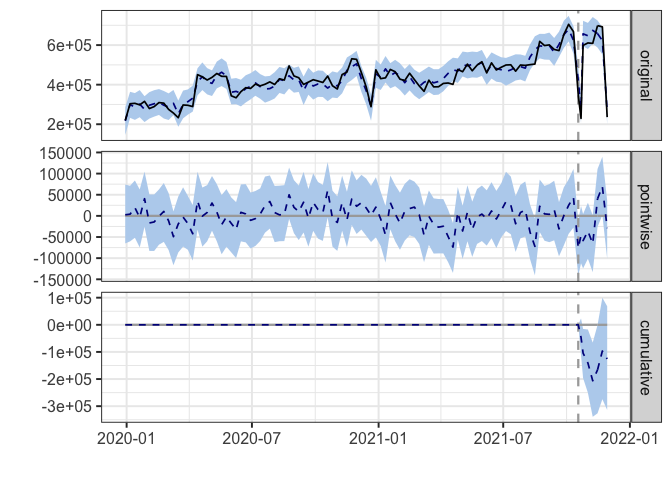
\includegraphics{t1_files/figure-latex/unnamed-chunk-1-1.pdf}

\begin{Shaded}
\begin{Highlighting}[]
\DocumentationTok{\#\#\#\#\#\#\# T1 \#\#\#\#\#\#}
\CommentTok{\# CM}
\NormalTok{cm\_t1 }\OtherTok{\textless{}{-}} \FunctionTok{read.csv}\NormalTok{(}\StringTok{"weekly\_pv\_cm\_t1.csv"}\NormalTok{, }\AttributeTok{sep =} \StringTok{\textquotesingle{},\textquotesingle{}}\NormalTok{,}\AttributeTok{header =} \ConstantTok{TRUE}\NormalTok{)}
\NormalTok{cm\_t1 }\OtherTok{\textless{}{-}}\NormalTok{ cm\_t1[}\FunctionTok{order}\NormalTok{(cm\_t1}\SpecialCharTok{$}\NormalTok{period, }\AttributeTok{decreasing=}\ConstantTok{TRUE}\NormalTok{), ]}
\NormalTok{cm\_t1 }\OtherTok{\textless{}{-}}\NormalTok{ cm\_t1[}\FunctionTok{order}\NormalTok{(cm\_t1}\SpecialCharTok{$}\NormalTok{week), ]}
\CommentTok{\#head(cm\_t1)}
\CommentTok{\#dim(cm\_t1)}

\CommentTok{\# Construct control and test cm\_t1}
\NormalTok{cm\_t1[,}\DecValTok{1}\NormalTok{] }\OtherTok{\textless{}{-}} \FunctionTok{as.Date}\NormalTok{(cm\_t1[,}\DecValTok{1}\NormalTok{],  }\AttributeTok{format=}\StringTok{"\%Y{-}\%m{-}\%d"}\NormalTok{)}
\FunctionTok{head}\NormalTok{(cm\_t1)}
\end{Highlighting}
\end{Shaded}

\begin{verbatim}
##         week period  C1_pv  C2_pv  T1_pv  T2_pv    C1_cm    C2_cm    T1_cm
## 1 2019-12-30    pre 172073 151800 210841 199453 29315.71 35947.70 32977.13
## 2 2020-01-06    pre 236933 181559 258295 235613 34505.40 40945.60 35977.70
## 3 2020-01-13    pre 233835 182458 242251 226282 47876.14 41901.76 37096.11
## 4 2020-01-20    pre 235297 198188 321493 234953 37328.79 38033.40 21160.58
## 5 2020-01-27    pre 227889 181722 294864 231657 41647.22 38298.21 37087.92
## 6 2020-02-03    pre 198485 176194 218892 222952 35901.39 48460.33 41818.96
##      T2_cm
## 1 23738.75
## 2 34191.56
## 3 39127.26
## 4 37952.44
## 5 39109.32
## 6 46779.60
\end{verbatim}

\begin{Shaded}
\begin{Highlighting}[]
\CommentTok{\# Define date }
\NormalTok{times}\OtherTok{=}\FunctionTok{as.Date}\NormalTok{(cm\_t1[,}\DecValTok{1}\NormalTok{])}
\NormalTok{pre.period }\OtherTok{\textless{}{-}} \FunctionTok{c}\NormalTok{(}\FunctionTok{min}\NormalTok{(}\FunctionTok{which}\NormalTok{(cm\_t1}\SpecialCharTok{$}\NormalTok{period}\SpecialCharTok{==}\StringTok{\textquotesingle{}pre\textquotesingle{}}\NormalTok{)), }\FunctionTok{max}\NormalTok{(}\FunctionTok{which}\NormalTok{(cm\_t1}\SpecialCharTok{$}\NormalTok{period}\SpecialCharTok{==}\StringTok{\textquotesingle{}pre\textquotesingle{}}\NormalTok{)))}
\NormalTok{post.period }\OtherTok{\textless{}{-}} \FunctionTok{c}\NormalTok{(}\FunctionTok{min}\NormalTok{(}\FunctionTok{which}\NormalTok{(cm\_t1}\SpecialCharTok{$}\NormalTok{period}\SpecialCharTok{==}\StringTok{\textquotesingle{}post\textquotesingle{}}\NormalTok{)), }\FunctionTok{max}\NormalTok{(}\FunctionTok{which}\NormalTok{(cm\_t1}\SpecialCharTok{$}\NormalTok{period}\SpecialCharTok{==}\StringTok{\textquotesingle{}post\textquotesingle{}}\NormalTok{)))}


\NormalTok{X }\OtherTok{=}\NormalTok{ cm\_t1[, }\DecValTok{3}\SpecialCharTok{:}\DecValTok{8}\NormalTok{, }\DecValTok{10}\NormalTok{]}
\NormalTok{y }\OtherTok{=}\NormalTok{ cm\_t1[, }\DecValTok{9}\NormalTok{]}
\CommentTok{\# cm\_t1 is (test, control, date)}
\NormalTok{fit\_cm\_t1}\OtherTok{=}\FunctionTok{zoo}\NormalTok{(}\FunctionTok{cbind}\NormalTok{(y, X),times)}
\CommentTok{\# Model fit}
\NormalTok{impact }\OtherTok{\textless{}{-}} \FunctionTok{CausalImpact}\NormalTok{(fit\_cm\_t1,times[pre.period] , times[post.period])}

\FunctionTok{summary}\NormalTok{(impact)}
\end{Highlighting}
\end{Shaded}

\begin{verbatim}
## Posterior inference {CausalImpact}
## 
##                          Average          Cumulative      
## Actual                   33776            236431          
## Prediction (s.d.)        35093 (2688)     245654 (18816)  
## 95% CI                   [29855, 40393]   [208982, 282750]
##                                                           
## Absolute effect (s.d.)   -1318 (2688)     -9223 (18816)   
## 95% CI                   [-6617, 3921]    [-46320, 27448] 
##                                                           
## Relative effect (s.d.)   -3.8% (7.7%)     -3.8% (7.7%)    
## 95% CI                   [-19%, 11%]      [-19%, 11%]     
## 
## Posterior tail-area probability p:   0.31159
## Posterior prob. of a causal effect:  69%
## 
## For more details, type: summary(impact, "report")
\end{verbatim}

\begin{Shaded}
\begin{Highlighting}[]
\FunctionTok{summary}\NormalTok{(impact, }\StringTok{"report"}\NormalTok{)}
\end{Highlighting}
\end{Shaded}

\begin{verbatim}
## Analysis report {CausalImpact}
## 
## 
## During the post-intervention period, the response variable had an average value of approx. 33.78K. In the absence of an intervention, we would have expected an average response of 35.09K. The 95% interval of this counterfactual prediction is [29.85K, 40.39K]. Subtracting this prediction from the observed response yields an estimate of the causal effect the intervention had on the response variable. This effect is -1.32K with a 95% interval of [-6.62K, 3.92K]. For a discussion of the significance of this effect, see below.
## 
## Summing up the individual data points during the post-intervention period (which can only sometimes be meaningfully interpreted), the response variable had an overall value of 236.43K. Had the intervention not taken place, we would have expected a sum of 245.65K. The 95% interval of this prediction is [208.98K, 282.75K].
## 
## The above results are given in terms of absolute numbers. In relative terms, the response variable showed a decrease of -4%. The 95% interval of this percentage is [-19%, +11%].
## 
## This means that, although it may look as though the intervention has exerted a negative effect on the response variable when considering the intervention period as a whole, this effect is not statistically significant, and so cannot be meaningfully interpreted. The apparent effect could be the result of random fluctuations that are unrelated to the intervention. This is often the case when the intervention period is very long and includes much of the time when the effect has already worn off. It can also be the case when the intervention period is too short to distinguish the signal from the noise. Finally, failing to find a significant effect can happen when there are not enough control variables or when these variables do not correlate well with the response variable during the learning period.
## 
## The probability of obtaining this effect by chance is p = 0.312. This means the effect may be spurious and would generally not be considered statistically significant.
\end{verbatim}

\begin{Shaded}
\begin{Highlighting}[]
\FunctionTok{plot}\NormalTok{(impact)}
\end{Highlighting}
\end{Shaded}

\includegraphics{t1_files/figure-latex/unnamed-chunk-2-1.pdf}

\end{document}
